\documentclass[10pt,a4paper]{article}
\usepackage{multicol}
\usepackage{a4wide}
\usepackage{xspace}
\usepackage[%
		pdfauthor={MeFoSyLoMa},%
		pdftitle={Petri Nets 2021 Call for papers},
	colorlinks=true,
	urlcolor=blue,
	]{hyperref}
\usepackage{nth}
\usepackage{graphicx}
\usepackage[utf8]{inputenc}
\usepackage[T1]{fontenc}
\usepackage{enumitem}
\usepackage{tikz}

\usetikzlibrary{calc}
\definecolor{couleurLoVe}{cmyk}{0, .19, .94, .0118}

\addtolength{\textwidth}{5.3cm}
\addtolength{\oddsidemargin}{-2.8cm}
\addtolength{\topmargin}{-3.5cm}
\addtolength{\textheight}{7cm}

\hypersetup{urlcolor=blue}
\setlist{noitemsep}
\newcommand{\styleUniv}[1]{\textcolor{black!75}{#1}}

\begin{document}
\mbox{}

\vspace{-1cm}\hspace{-1.5cm}\includegraphics[width=1.1\textwidth]{images/bandeau.png}
\begin{multicols}{2}
\begin{center}
{\large\bf
Call for Papers and Announcement\\
Petri Nets 2021

\bigskip

\nth{42} INTERNATIONAL CONFERENCE\\
ON APPLICATION AND THEORY OF \\
PETRI NETS AND CONCURRENCY

\smallskip

\& special track on Application of Concurrency to System Design (ACSD)
\bigskip

21--25 June 2021, Paris, France}

\bigskip

Additional information about the conference will be published via
\url{http://conf-2021.petrinet.net}

\smallskip

Contact: \href{mailto:pn2021@petrinet.net}{pn2021@petrinet.net}
\end{center}

\columnbreak

\begin{center}
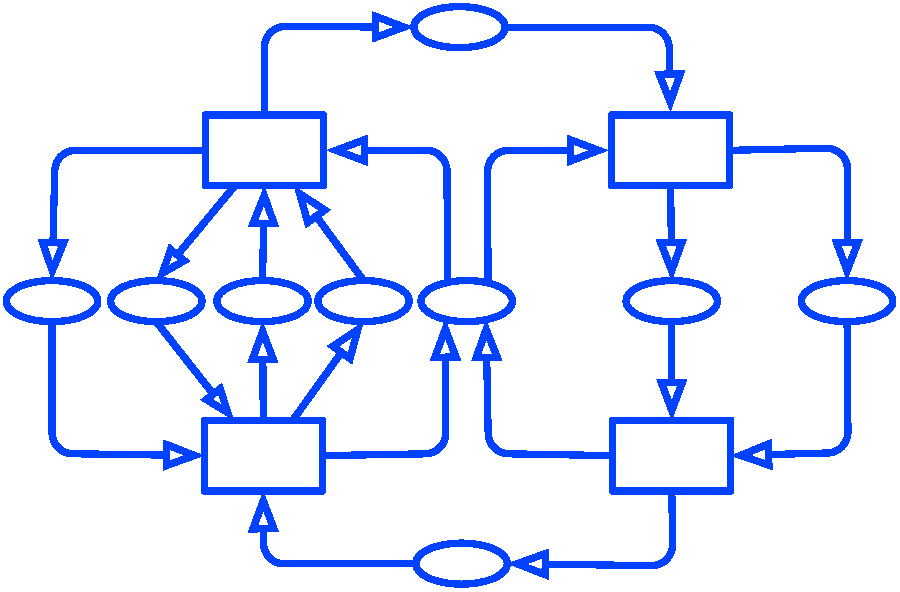
\includegraphics[height=2.5cm]{logos/LogoPN.pdf}

{\bf Important dates:}

\begin{tabular}{|l|r@{, 2021 }l|}
\hline
Abstract submission & January 13 & (*) \\
\hline
Submission of papers & January 20 & (*) \\
\hline
Notification & March 5 & \\
\hline
Final version due & March 19 & (*) \\
\hline
Participation in Tool Exhibition & May 31 & \\
\hline
Workshops and Tutorials & June 21--22 & \\
\hline
Main Conference & June 23--25 & \\
\hline
\end{tabular}

{\small (*) The deadline is the end of day Anywhere on Earth (\href{https://en.wikipedia.org/wiki/Anywhere_on_Earth}{AoE})}
\end{center}
\end{multicols}

\bigskip

The {\bf\nth{42} annual international Petri Nets conference} will be organised by
the {\bf LoVe (Logics and Verification) team} of the computer science laboratory 
{\bf \href{https://lipn.univ-paris13.fr/}{LIPN} (Laboratoire d'Informatique de Paris
Nord), University Sorbonne Paris Nord and CNRS},
jointly with members of the {\bf Paris region \href{http://mefosyloma.fr/}{MeFoSyLoMa} group (Méthodes Formelles
pour les Systèmes Logiciels et Matériels)}.
%
The conference will take place at the
\href{https://www.mshparisnord.fr}{\bf Maison des Sciences de l'Homme},
which fosters and promotes research in humanities and social sciences.
%
The language of the conference is English, and its proceedings will be published by
{\bf Springer-Verlag in Lecture Notes in Computer Science}.
Papers presenting {\bf original research on application or theory of Petri nets}, as well
as contributions addressing topics relevant to the general field of {\bf distributed and
concurrent systems} are sought. Authors from the {\bf applications of concurrency
to systems
design} are encouraged to submit to this special track. All accepted papers will be considered for an {\bf ``Outstanding
Paper''} award. Authors of {\bf selected papers} presented at the conference will be invited
to submit an extended version that will be further reviewed for inclusion into a special
issue of {\bf Fundamenta Informaticae}.

\begin{multicols}{2}
\paragraph*{General topics related to concurrency:}\mbox{}

% \vspace*{-0.3cm}
\begin{itemize}
\item Model checking and verification of distributed systems
\item Verification of infinite-state or parametric systems
\item Causality/partial order theory of concurrency
\item Educational issues related to concurrency
\item New developments in the theory of concurrency
\item Modelling of hardware and biological systems
\end{itemize}

\vspace*{-0.5cm}
\paragraph*{Special track on ACSD (Application of Concurrency to System Design)}
Both theoretical and applied research about formal approaches (in a broad sense) to designing computer systems that exhibit concurrent behaviour.
The formal models of computation and concurrency for the above systems and problems are not limited by Petri nets, but also include models like dataflow models, communicating automata, process algebras, graph rewriting systems, state charts, MSCs, modal and temporal logics.

% \smallskip
% \bigskip
% \bigskip

\begin{center}
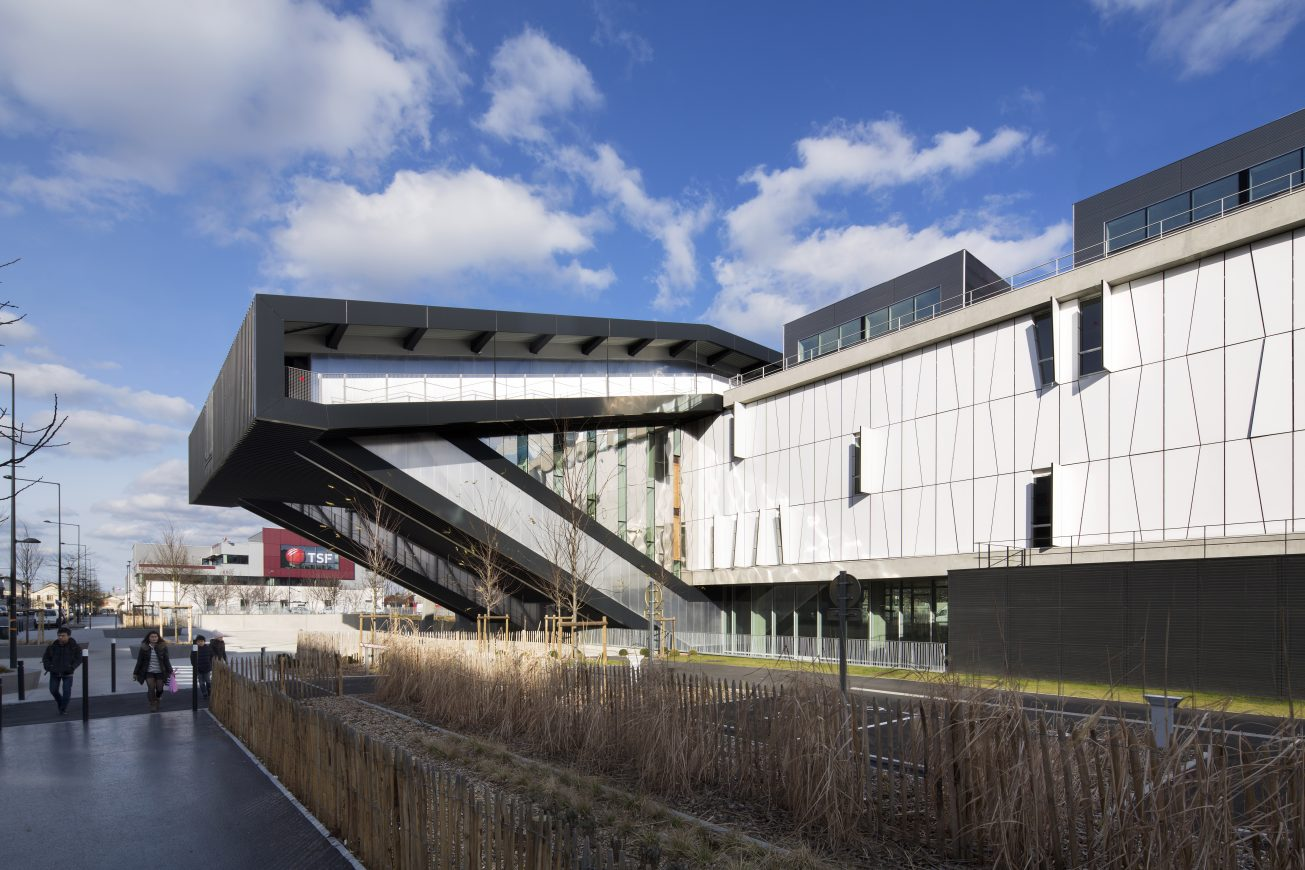
\includegraphics[scale=0.19]{images/MSH.jpg}
\end{center}
\columnbreak

\paragraph*{Topics specific to Petri Nets:}\mbox{}

% \vspace*{-0.3cm}
\begin{itemize}
\item Analysis and synthesis, structure and behaviour of nets
\item System design and model-driven development using nets
\item Relationships between Petri nets and other approaches
\item Net-based semantical, logical and algebraic calculi
\item Higher-level net models (coloured nets, timed nets, etc.)
\item Stochastic net models
\item Verification and model checking using nets
\item Process discovery and conformance checking
\item Computer tools for nets
\item Standardisation of nets
\item Experience reports describing applications of nets to different kinds of systems
and application fields, e.g.:

	\begin{tabular}{ll}
	flexible manufacturing systems & office automation \\
	real-time systems & workflows \\
	embedded systems & process mining \\
	biological systems & supervisory control \\
	health and medical systems & protocols and networks \\
	environmental systems & Internet and Web services \\
	hardware & e-commerce and trading \\
	telecommunications & programming languages \\
	railway networks & performance evaluation \\
	component based development & operations research \\
	\end{tabular}
\end{itemize}
\end{multicols}

\begin{tikzpicture}[remember picture,overlay]
	\node [minimum width=\paperwidth, 
            minimum height=2cm,
            fill=couleurLoVe
          ] at ($(current page.south west)+(0.5\paperwidth,0.4)$) {};
	\node at ($(current page.south west)+(0.5\paperwidth,0.7)-(8,0)$) {
		\begin{minipage}{6em}
			
\includegraphics[height=1cm]{logos/logo-lipn-plein.png}
		\end{minipage}
	};
	\node at ($(current page.south west)+(0.5\paperwidth,0.7)-(6,0)$) {
		\begin{minipage}{6em}
			
\includegraphics[height=1cm]{logos/logoup13_noir.png}
		\end{minipage}
	};
	\node at ($(current page.south west)+(0.5\paperwidth,0.7)-(2.5,0)$) {
		\begin{minipage}{6em}
			
\includegraphics[height=1cm]{logos/logo-MSHParisNord.jpg}
		\end{minipage}
	};
	\node at ($(current page.south west)+(0.5\paperwidth,0.7)+(0.5,0)$) {
		\begin{minipage}{6em}
			
\includegraphics[height=1cm]{logos/logo-cnrs.pdf}
		\end{minipage}
	};
	\node at ($(current page.south west)+(0.5\paperwidth,0.7)+(2.5,0)$) {
		\begin{minipage}{6em}
			
\includegraphics[height=1cm]{logos/mefosyloma.png}
		\end{minipage}
	};
	\node at ($(current page.south west)+(0.5\paperwidth,0.7)+(5,0)$) {
		\begin{minipage}{6em}
			
\includegraphics[height=1cm]{logos/logo-idf.png}
		\end{minipage}
	};
	\node at ($(current page.south west)+(0.5\paperwidth,0.7)+(9,0)$) {
		\begin{minipage}{6em}
			
\includegraphics[height=1cm]{logos/logo_RFSI.png}
		\end{minipage}
	};
\end{tikzpicture}
\newpage
\mbox{}

\vspace*{-2em}
\paragraph*{Paper Submission:}\mbox{}

Two kinds of papers can be submitted:
\vspace*{-0.2cm}
\begin{itemize}
\item {\bf Regular papers (max.\ 20 pages excluding references)} describing original results pertaining
to the development of the theory of Petri nets and distributed and concurrent systems in
general, new results extending the applicability of Petri nets, or case studies, application
and experience reports pertinent to the practical use of Petri nets and concurrency.
\item {\bf Tool papers (max.\ 10 pages excluding references)} describing a computer tool based on Petri
nets (not an application of the tool or the theory behind the tool). The tool should
be available for use by other groups (but not necessarily for free). The submission
should indicate how the reviewers can get access to the tool (this must be for free).
The tool will be demonstrated in the Tool Exhibition, in addition to being presented
in a conference talk.
\end{itemize}

\vspace*{-0.2cm}
\noindent Papers must be written in English using the Springer LNCS format: \url{http://www.springer.de/comp/lncs/authors.html},
including line numbers (\emph{e.g.} \texttt{lineno} \LaTeX{} package)
and submitted electronically (as a PDF file) by the deadline indicated at the top
of this Call for Papers using EasyChair:
% 
% {\centering
	\url{https://easychair.org/conferences/?conf=petrinets2021}
% }

\vspace*{-0.5em}
\paragraph*{Tool Exhibition:}\mbox{}

An exhibition of Petri net tools will take place on Wednesday. It consists of informal
demonstrations for small groups/individuals and there are no scheduled talks. Requests
for participation in the tool exhibition must be sent to the Tool Exhibition chairs
by the deadline stated at the top of this Call for Papers. They should include a link
to the Web pages for the tool (or a short description of the tool). The demonstrators
should bring their own laptops, while the organisers may be requested to give access
to the Internet.

\vspace*{-0.5em}
\paragraph*{Courses, Workshops and Tutorials:}\mbox{}

The main conference takes place from Wednesday~23 to Friday~25.
The three days before the main conference also offer a wide range of activities.
The {\bf Petri Net Course}
takes place from Sunday~20 to Tuesday~22.
It offers a thorough introduction to Petri nets in
four half-day modules on Sunday~20 and Monday 21, and a full-day tutorial module on Tuesday~22.
For successful participation in the entire course, including preparation and examination,
three credit points (ECTS) will be awarded. Each module of the course can also be
taken separately, without any credit.
% The main conference takes place from Wednesday to Friday. The two days before the
% main conference also offer a wide range of activities:
% \vspace*{-0.2cm}
% \begin{itemize}
% \item \textbf{Courses} and \textbf{Tutorials} on applications of Petri nets and/or
% new developments
% presented
% by experts in the area. The courses and the tutorials can be followed independently
% of one another.
% \item \textbf{Workshops} also take place on Monday and Tuesday.
% \end{itemize}
Detailed descriptions of Workshops and Tutorials will be made available via the conference
Web pages.

It is also possible to arrange {\bf Meetings} and {\bf Courses} related to Petri Nets.
Submissions for such activities must contain a 2--5 page description. They must be
received by the Workshops and Tutorials chairs via email no later than January 10,
2021.

\subsection*{Organisation}

\vspace*{-1em}
\setlength{\columnsep}{-5cm}
\begin{multicols}{2}
\paragraph*{Programme Committee co-chairs:}\mbox{}

\noindent Didier Buchs \\
\indent \styleUniv{University of Geneva, Switzerland} \\
\noindent Josep Carmona \\
\indent \styleUniv{Universitat Politècnica de Catalunya, Spain} \\
\noindent Jörg Desel (ACSD track) \\
\indent \styleUniv{FernUniversität in Hagen, Germany} \\
\noindent Alex Yakovlev (ACSD track) \\
\indent \styleUniv{University of Newcastle-upon-Tyne, UK} \\
\href{mailto:pn2021-PC@petrinet.net}{pn2021-PC@petrinet.net}

\vspace*{-0.5em}
\paragraph*{Workshops co-chairs:}\mbox{}

\noindent Gianfranco Ciardo \\
\indent \styleUniv{Iowa State University, USA} \\
\noindent Daniel Moldt \\
\indent \styleUniv{Universität Hamburg, Germany} \\
\noindent Thomas Châtain (organisation) \\
\indent \styleUniv{LSV, CNRS, ENS Paris-Saclay, France} \\
\href{mailto:pn2021-WT@petrinet.net}{pn2021-workshops@petrinet.net}

\vspace*{-0.5em}
\paragraph*{General chairs:}\mbox{}

\noindent Laure Petrucci \\
\indent \styleUniv{LIPN, CNRS, \\ \indent Université Sorbonne Paris Nord, France}\\
\noindent Étienne André \\
\indent \styleUniv{LORIA, CNRS, \\ \indent Université de Lorraine, France} \\
\href{mailto:pn2021@petrinet.net}{pn2021@petrinet.net}

\vspace*{-0.5em}
\paragraph*{Tool exhibition chairs:}\mbox{}

\noindent Benoît Barbot \\
\indent \styleUniv{LACL, Université Paris 12, France} \\
\noindent Alexandre Duret-Lutz \\
\indent \styleUniv{LRDE, EPITA, France} \\
\href{mailto:pn2021-tool@petrinet.net}{pn2021-tool@petrinet.net}

\mbox{}

\columnbreak

\paragraph*{Steering committee:}\mbox{}

\vspace*{-1em}
\setlength{\columnsep}{0.2cm}
\begin{multicols}{2}
\noindent W. van der Aalst, Germany\\
G. Ciardo, USA\\
J. Desel, Germany\\
S. Donatelli, Italy\\
S. Haddad, France\\
K. Hiraishi, Japan\\
J. Kleijn, The Netherlands\\
F. Kordon, France\\
M. Koutny, UK (chair)\\

\columnbreak

\noindent L. M. Kristensen, Norway\\
C. Lin, China\\
W. Penczek, Poland\\
L. Pomello, Italy\\
W. Reisig, Germany\\
G. Rozenberg, The Netherlands\\
M. Silva, Spain\\
A. Valmari, Finland\\
A. Yakovlev, UK\\
\end{multicols}

\paragraph*{Programme committee:}\mbox{}
\vspace*{-1em}
\begin{multicols}{2}
\noindent Elvio Amparore, Italy \\
Abel Armas Cervantes, Australia \\
Paolo Baldan, Italy \\
Benoît Barbot, France \\
Béatrice Bérard, France \\
% Didier Buchs, Switzerland \\
% Josep Carmona, Spain \\
Thomas Chatain, France \\
% Jörg Desel, Germany \\
Raymond Devillers, Belgium \\
Susanna Donatelli, Italy \\
Boudewijn van Dongen, The Netherlands \\
Javier Esparza, Germany \\
David de Frutos Escrig, Spain \\
Stefan Haar, France \\
Xudong He, USA \\
Loïc Helouet, France \\
Marieke Huisman, The Netherlands \\
Ryszard Janicki, Canada \\

\columnbreak

\noindent 
Anna Kalenkova, Australia \\
Jörg Keller, Germany \\
Michael Köhler-Bußmeier, Germany \\
Irina Lomazova, Russia \\
Robert Lorenz, Germany \\
Roland Meyer, Germany \\
{\L}ukasz Mikulski, Poland \\
Andrew Miner, USA \\
Andrey Mokhov, UK\\
Marco Montali, Italy \\
Jaco van de Pol, Denmark \\
Dumitru Potop, France\\
Pierre-Alain Reynier, France \\
Arnaud Sangnier, France \\
Natalia Sidorova, The Netherlands \\
% Alex Yakovlev, UK \\
W{\l}odek Zuberek, Canada \\
% ADDED BY ÉTIENNE TO MAKE SURE WHICH VERSION WE TALK ABOUT
{\tiny \textcolor{black!2}{Version: \today{}}}
\end{multicols}
\end{multicols}

\begin{tikzpicture}[remember picture,overlay]
	\node [minimum width=\paperwidth, 
            minimum height=2cm,
            fill=couleurLoVe
          ] at ($(current page.south west)+(0.5\paperwidth,0.4)$) {};
	\node at ($(current page.south west)+(0.5\paperwidth,0.7)-(8,0)$) {
		\begin{minipage}{6em}
			
\includegraphics[height=1cm]{logos/logo-lipn-plein.png}
		\end{minipage}
	};
	\node at ($(current page.south west)+(0.5\paperwidth,0.7)-(6,0)$) {
		\begin{minipage}{6em}
			
\includegraphics[height=1cm]{logos/logoup13_noir.png}
		\end{minipage}
	};
	\node at ($(current page.south west)+(0.5\paperwidth,0.7)-(2.5,0)$) {
		\begin{minipage}{6em}
			
\includegraphics[height=1cm]{logos/logo-MSHParisNord.jpg}
		\end{minipage}
	};
	\node at ($(current page.south west)+(0.5\paperwidth,0.7)+(0.5,0)$) {
		\begin{minipage}{6em}
			
\includegraphics[height=1cm]{logos/logo-cnrs.pdf}
		\end{minipage}
	};
	\node at ($(current page.south west)+(0.5\paperwidth,0.7)+(2.5,0)$) {
		\begin{minipage}{6em}
			
\includegraphics[height=1cm]{logos/mefosyloma.png}
		\end{minipage}
	};
	\node at ($(current page.south west)+(0.5\paperwidth,0.7)+(5,0)$) {
		\begin{minipage}{6em}
			
\includegraphics[height=1cm]{logos/logo-idf.png}
		\end{minipage}
	};
	\node at ($(current page.south west)+(0.5\paperwidth,0.7)+(9,0)$) {
		\begin{minipage}{6em}
			
\includegraphics[height=1cm]{logos/logo_RFSI.png}
		\end{minipage}
	};
\end{tikzpicture}
\end{document}
